%%%%%%%%%%%%%%%%%%%%%%%%%%%%%%%%%%%%%%%%%%%%%%%%%%%
% System Design - Microservices
%%%%%%%%%%%%%%%%%%%%%%%%%%%%%%%%%%%%%%%%%%%%%%%%%%%
\chapter{System Design}

A Microservice Architecture is employed to create the application as a series of distinct interactive components. A Mono Repository Model\cite{monorepository} has been adopted as to increase developer productivity and mitigate the complexities of code sharing across various different repositories.

\section{What are Microservices?}
The term "Microservice" does not hold a true or set definition it is merely a term introduced by a number of software architects at a workshop near Venice in May, 2011 to provide context to a number of reoccurring design principles and patterns that seemed to be emerging more frequently.
	Just under a year later, James Lewis presented at 33rd Degree, conference for Java Masters in Krakow where he spoke about building systems composed of systems and focusing on the Unix philosophy of minimalist and modular. \cite{JamesLewis33rdDegree} 
This gave rise to the hot new term "Microservices" and began to get more and more attention. 

Martin Fowler describes the Microservice Architectural style as a approach to developing a single application as a suite of independently deployable services each running in its own process \cite{MicroservicesResourceGuide}. Each service should be independent in its our right and provide functionality based around a single responsibility. Services should be loosely coupled, provide high cohesion and adhere to the single responsibility principle. All of a sudden it can be seen that many of the traits mentioned are key concepts in Object Orientated Programming which are also common in the design principles of Service Orientated Architecture. Stubbings and Polovina \cite{StubbingsPolovina} explore and contrast the how Object Orientated expertise can be leveraged in the design of Service Orientated Architecture (SOA). Employing fundamental aspects of the Object Orientated Programming paradigm such as abstraction and encapsulation can provide a significantly more proficient approach to designing Microservice based applications.

\section{Are Microservices just SOA?}

This immediately sparks the debate - Is Microservice Architecture really just SOA? Upon the rise of the term "Microservices" into the community, many SOA architects and engineers were coming forward, saying "We've been doing this for years!". And as Martin Fowler mentions in his keynote\cite{GOTOConference} - "Service Orientated Architecture is a very broad term". It encompasses a vast landscape of design concepts, principles, patterns and implementation standards. And it is often considered controlled by vendors who release commercial solutions Fowler goes on to mention that in essence Microservices can be really be considered a subset of SOA.

Indeed, this is a popular and well defined statement and is backed up by Adrian Cockcroft, the man responsible for pioneering the architectural style at Netflix as they moved towards cloud based and Microservice orientated design. He describes the architecture as "fine-grained SOA", in his keynote at Dockercon in 2014 \cite{adriancockcroft}.

Netflix are widely considered to be part of the pioneers of the Microservice Architectural style and have helped pave the way for it to flourish, introducing such libraries and tools as Hystrix\cite{Hystrix} and Chaos Monkey\cite{ChaosMonkey} for testing and strengthening systems.

\section{Monolith vs MicroServices}

Josh Evans of Netflix provides the analogy of the human body to describe the architectural style in his keynote \cite{MasteringChaosNetflix}. He describes Microservices as the organs which make up the human body and work together as one organism.
Perhaps the best way to put Microservices into context is by comparing the differences in contrast to a traditional monolithic architecture. Martin Fowler uses a similar example in his Resource Guide to Microservices where he outlines a potential structure of a traditional enterprise application. \cite{MicroservicesResourceGuide} Take for example a simple application that exists in 3 tiers.

% Subsection - Presentation Layer ----------------------
\subsection{Presentation Layer}
A Presentation Layer sits at the top of the application. This is the entry point of an application from a customer or user perspective, more commonly referred to as the front end. For example, this layer may consist of a web application composed of HTML, CSS and Javascript presenting a user interface to the client. 

% Subsection - Logic Layer -----------------------------
\subsection{Logic Layer}
A Logic Layer lies behind the user interface and provides functionality to carry out business operations. This could be a wide variety of functionality and responsibilities could be anything from user accounts to instant messaging to calendar events. For this purpose, lets take a Java server application as the example. Requests may be issues over HTTP via REST\cite{Fielding:2000:ASD:932295} or RPC and handled accordingly by a number of object orientated classes to perform the requested operation.

% Subsection - Data Layer ------------------------------
\subsection{Data Layer}
The Data Layer lives at base of the application stack and is responsible for persistence of the raw application data. All of the data needed and in use by the application exists here. A data store such as a relational database could be employed to persist and manage data in this layer. The server application may employ a framework such as Hibernate\cite{JPAHibernate} JPA for object relational mapping in order to perform actions on data. 

The monolith in this example is the server application. The services it provides run on a single process and are not independently deployable. A monolith is a software application whose modules cannot be executed independently \cite{MicroservicesYesterdayTodayTomorrow}. In the case of the example defined above we may need to make improvements, changes or simple bug fixes to any one of the services we described. Changes made to the source code of the application imply - rebuild and redeploy. But what if the changes are small and confined to one service? There is an overhead associated with this as it becomes expensive to build a new release for production and this may only be affordable every couple of weeks. Continuous integration and continuous deployment are considered hidden dividends of Microservices \cite{hiddendividends}. Although not exclusive to the world of Microservices they may in theory be more easily orchestrated as each service has a single responsibility, however require careful orchestration. This allows developers to focus on developing and can speed up productivity across teams. 

% Section - Microservices Characteristics
\section{Microservices Characteristics}

To migrate the example above to a Microservice based architecture the functionality described for handling user accounts, instant messaging and calendar events would be refactored into individual services that are independently deployable and each run in an isolated process. This provides a more loosely coupled and highly cohesive design, adhering more so to the single responsibility principle mentioned previously. However, that being said this does not mean it is an easy task to move from one architecture to another. Particularly in the case of Microservices there a wide range of aspects to be taken into consideration. Knoche writes of using modernization paths to predict performance impact on systems migrating from monolithic software applications towards microservices \cite{Knoche:2016:SRP:2851553.2892039}.
Microservices may not hold a definition set in stone however, it is clear that there is a number of definitive common characteristics that can be used to identify with architectural style.

% Independent Deployment
\subsection*{ 1. Independent Deployment }
Independent deployment is a key characteristic and indeed perhaps the most important principle of Microservice architecture. The idea of having the ability to deploy services as independent applications implies a number of benefits.

\subsubsection*{Language Neutrality}
A collection of Microservices operating together for the purpose of a single application do not have to be confined to one programming language. Sam Newmann uses the term - Technology Heterogeneity \cite{BuildingMicroServices}. A service can use the best tools for the job and there may be various services written in completely different languages using different technologies.

\subsubsection*{Specialised Teams}
Teams working on their respective services can become experts in the area and obtain a great understanding of how to carry out their jobs to the best of their ability. Having teams focus on their respective services may speed up productivity \cite{BuildingMicroServices}. Why be a jack of all trades and master of none?

\subsubsection*{Appropriate Scaling}
Independent Deployment lends itself to scaling in the right places. In terms of a traditional monolithic piece of software, the monolith may be replicated numerous times to achieve desired scaling. This infers the question - is every aspect of the system being used enough to justify increased scaling of the entire system. Independent deployment offers scaling of individual services where appropriate, the term horizontal scaling is used \cite{MasteringChaosNetflix}.

% Bounded Context
\subsection*{ 2. Bounded Context }

The term "Bounded Context" is used when describing the characteristics of Microservice Architecture. This pattern is key in Domain Driven Design \cite{BoundedContext}. Bounded context in Microservices refers to organisation and creation of services based upon their business logic. A service should have a single responsibility and that responsibility should be entirely encapsulated within that service. This also lends itself to the idea of specialised teams as previously mentioned. Fowler speaks in his keynote about how Amazon divided themselves into teams responsible for a section of business logic all the way through to the end-user experience \cite{GOTOConference}. 

% Communication
\subsection*{ 3. Communication }
In a cloud or distributed environment service interactions with one another can be carried out via IPC (inter-process communication) or protocols such as HTTP are commonly applied. Many Microservices communicating together in a chain through HTTP may suggest a certain amount of latency being involved, depending on what operations are being carried out. To combat situations like this, Google introduced gRPC\cite{gRPC}. gRPC is as open source RPC framework that employs Protocol buffers\cite{ProtocolBuffers} as a method of serializing structured data. It is highly efficient and is designed to target speed and performance. Binary data is sent through the wire at high speeds, alongside rapid serialisation/deserialization \cite{gRPCHackernoon}.

In order to provide communication via services or processes it is standard to use light-weight mechanisms \cite{MicroservicesYesterdayTodayTomorrow}. This also lends itself to the idea of smart endpoints and dumb pipes\cite{MicroservicesResourceGuide}. The services themselves become the endpoints where business logic lives and pipes refer to the mechanisms used for them to communicate which are kept simple.

% Decentralisation
\subsection*{ 4. Decentralisation }
Decentralisation of services infers a substantial amount of additional complexities within an application ecosystem. How does a client know what service it needs to contact in a cloud or distributed network? API Gateways\cite{APIGateways} and Service Discovery\cite{ServiceDiscovery} are two critical concepts in Microservice Architecture. An API Gateway uses a Facade pattern\cite{Gamma:1995:DPE:186897} from object orientated design to encapsulate how requests are made to a number a services. This minimises code complexity on the client side and eliminates direct calls to services made by the client. The API Gateway is used in conjunction with a Service Discovery pattern. This may be either client side or server side. Service Discovery employs the use of a service registry, a database of network locations of available service instances\cite{ServiceDiscovery}.

% Containerisation -------------------------------------
\section{Containerisation with Docker}
Docker \cite{Docker} is a containisation platform that utilises the host operating system using lightweight images at the application layer to build and ship applications effectively and quickly. Containers can be considered as instances of images  running in isolated processes. They are often compared to virtual machines however they are more lightweight and can share the host OS kernal with many other containers. Virtual machines often take a couple of minutes to start whereas containers launch in a number of seconds. Container images are substantially smaller than virtual machines and are typically tens of MBs in size. In the last number of years Docker has become an industry leader in the world of Microservice Architecture. Sinnott and Korzhirbayev carried out a comparison of container-based technologies for the cloud\cite{KOZHIRBAYEV2017175} where they analyse Docker and evaluate pros and cons of container-based technologies based on in depth research of a number of performance metrics such as CPU, Disk I/O and Network I/O performance.

My Consultancy Services aims to provide containerisation of all services throughout the application. For example, housed in the mono repository of the project is a number of sub directories each containing a distinct containerised service. Such as:

\begin{itemize}
\item{Accounts Service}
\item{Calendar Service}
\item{Accounts Database}
\item{CouchDB Per User}
\item{Calendar Server}
\end{itemize}


Each service is distinct in its own right and available throughout the Docker network at its own service URL.

\subsection{Dockerfiles and Docker Compose}

The system utilizes Dockerfiles and Docker Compose for container orchestration.

Containers are built with Docker using Dockerfiles\cite{dockerfile}. A Dockerfile is a declarative file in which instructions for images containing applications or services are defined. For example, a basic Dockerfile may include:

\begin{itemize}
\item
A base image

\item
Installation of Dependencies

\item
Adding of source code

\item
Exposing ports to the host OS

\item
Commands for starting an application
\end{itemize}

\subsection*{ Example Dockerfile }

\begin{minted}{Dockerfile}
# Base Image
FROM node:alpine

# Specify a working directory
WORKDIR /app

# Add package.json and install dependencies
ADD package.json /app/package.json
RUN npm install

# Add application source code
ADD . /app

# Expose port 3000 on host machine
EXPOSE 3000

# Start the server
CMD ["node", "server.js"]
\end{minted}

More detailed and complex configurations can also be defined such as environment variables and volumes. Volumes provide a way in which containers can persist data. Smart, Nguyen and Jaramillo provide excellent analysis of how Docker technology can be leveraged in Microservice Architecture \cite{LeveragingMicroservicesArchDocker}.

% Docker compose
Docker compose can be used for the orchestration of multiple containers specifying their build paths to each service's respective Dockerfile. Similar to Dockerfiles a number of configuration settings can be defined here. John Zaccone\cite{JohnZaccone}, a Docker Captain, provides an excellent example using Docker Compose in his keynote at Dockercon 2017, the source code of his demo application can be found on his Github \cite{dockercompose}.

\subsection{Containerised Development Environments}
Through the use of volumes, a \texttt{docker-compose.debug.yml} file can be defined which allows development in a containerised environment. It is essential to have a good understanding of how an application behaves in a containerised environment for production purposes and therefore taking the extra time to setup a development environment which closely mimics this is truly a beneficial endeavour. 

\subsection*{Example \texttt{docker-compose.debug.yml}}

\begin{minted}{yaml}
version: "3"

services:
    account-service-api:
        image: "account-service-api"
        build: .
        user: "node"
        working_dir: /home/node/app
        volumes:
            - .:/home/node/app
        ports:
            - "9000:9000"
            - "9229:9229" # Expose ports for debugging via Chrome Inspect
        depends_on:
            - "account-database"
            - "calendar-service-api"
            - "couchdb"
        command: "npm run watch"

    account-database:
        image: "account-database"
        build:
            context: ../account-database
        volumes:
            - db-data:/var/lib/postgresql/data
        ports:
            - "5432:5432"
        restart: always

    calendar-service-api:
        image: "calendar-service-api"
        build:
            context: "../calendar-service-api"
        ports:
            - "9001:9001"
        depends_on:
            - "radicale-caldav-server"
        command: "npm run start"

    couchdb:
        image: "couchdb"
        build:
            context: ../couchdb-per-user
        volumes:
            - couchdb-data:/opt/couchdb/data
        ports:
            - "5984:5984"
        restart: always

    couchdb-configurator:
        image: "couch-configurator"
        build:
            context: ../couchdb-per-user/configurator
        depends_on:
            - couchdb
        command: ["/wait-for-couchdb.sh", "couchdb", "5984", "/configure-couchdb.sh"]

    radicale-caldav-server:
        image: "radicale-caldav-server"
        build:
            context: "../radicale-caldav-server"
        ports:
            - "5232:5232"
        volumes:
            - cal-data:/home/radicale/data
            - config:/home/radicale/config
        restart: always

volumes:
    db-data:
    couchdb-data:
    cal-data:
    config:
\end{minted}

\section{Jenkins Pipeline}

A Jenkins Pipeline\cite{jenkinspipeline} has been setup for build stages and deployment.
Jenkins can be deployed on bare metal, VPS (Virtual Private Server) or as a Docker container and can be configured as a standalone server or in a cluster with Jenkins Swarm\cite{jenkinsSwarm}. The modus operandi employed by Delta Ready Technology is that of a Jenkins Swarm running in a Docker Swarm\cite{dockerswarm}. Essentially, Jenkins is deployed as a global service on a three node Docker Swarm which provides a degree of fault tolerance and redundancy.  Additionally, three Jenkins Agents which are used to perform the build are run globally across the cluster.  A custom Docker Registry is used to store the docker images built in the CI (Continuous Integration)\cite{CI} process and resides at
\url{https://registry.deltareadytechnology.com.au
} and is protected by User Access Control.

A build is triggered when a commit is made to the either of the Git branches \texttt{master} or \texttt{develop} in BitBucket.  The branches that trigger builds are configurable and currently a regular expression that tests for develop and master achieves the desired effect.  Rather than polling the BitBucket repository a Webhook (see Fig \ref{fig:webhooks}) is installed in BitBucket Cloud when configuring the Bitbucket Branch Source Plugin.

\begin{figure}
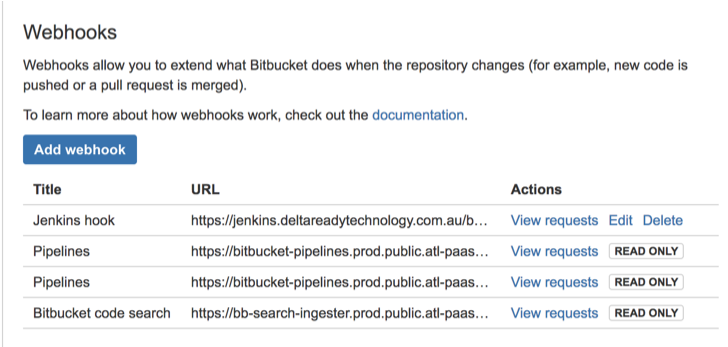
\includegraphics[width=\textwidth]{img/webhooks.png}
\caption{Webhooks}
\label{fig:webhooks}
\end{figure}


\begin{figure}
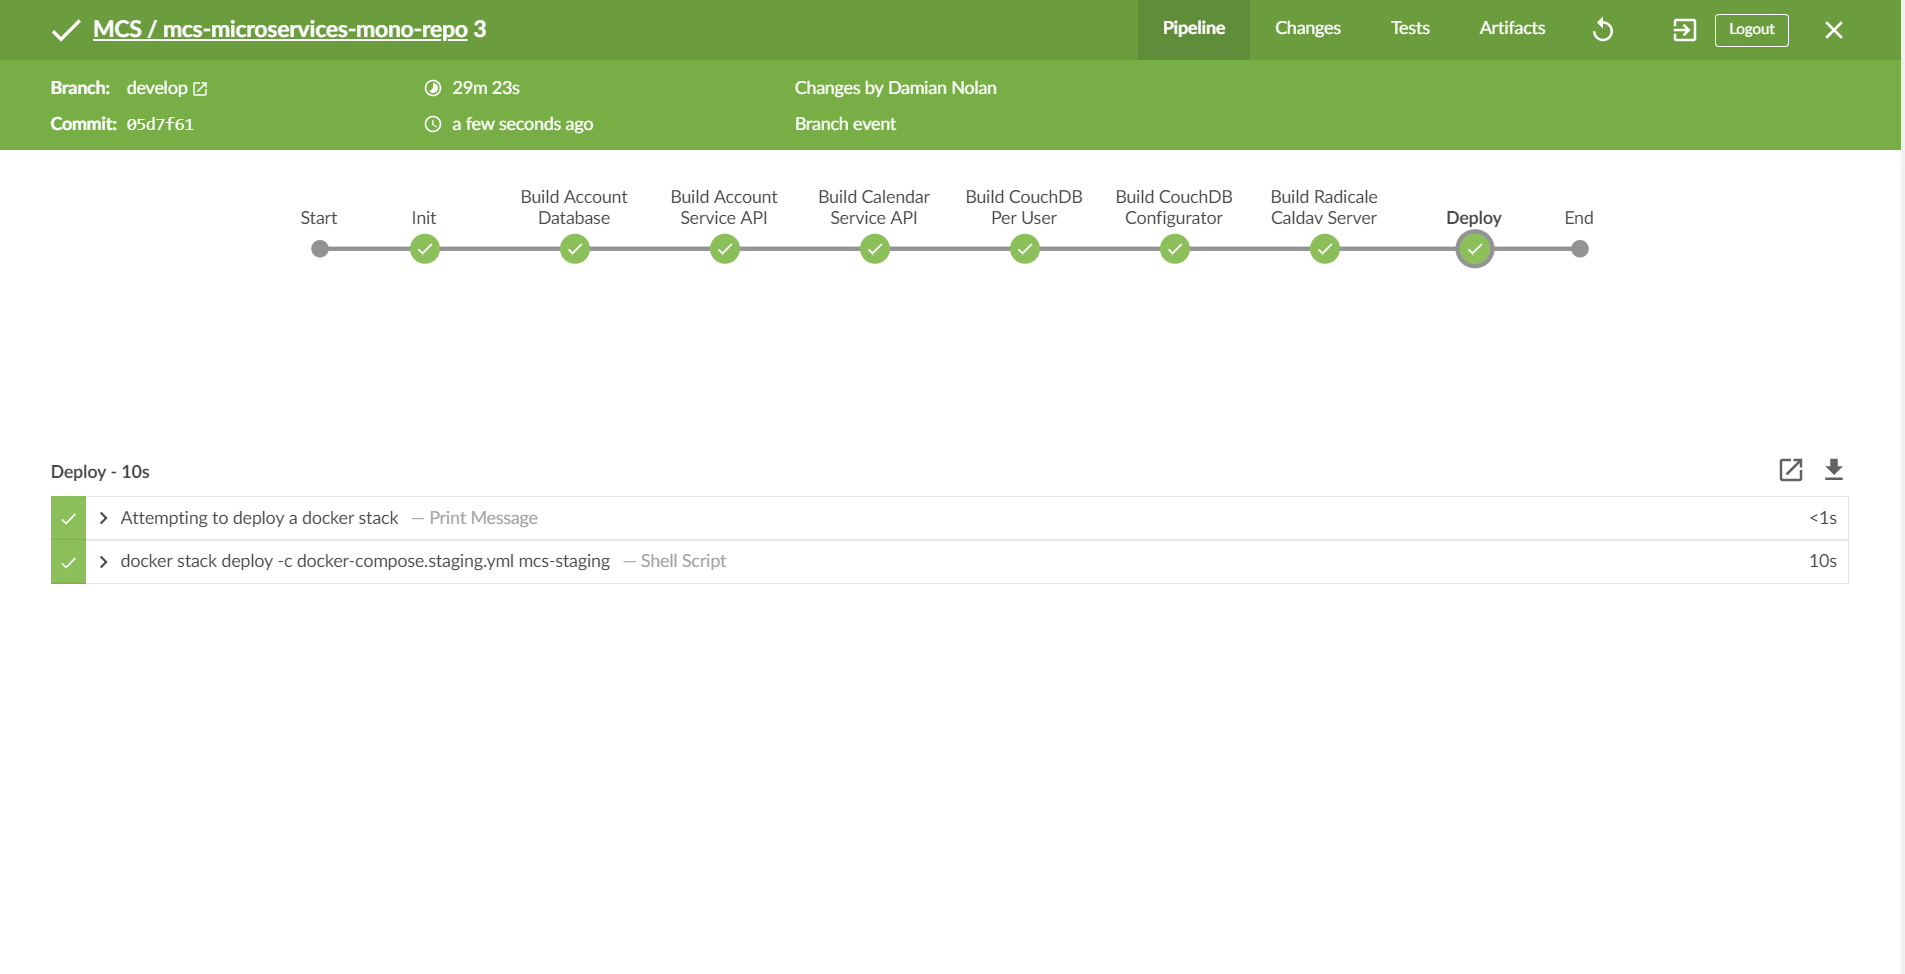
\includegraphics[width=\textwidth]{img/jenkins.png}
\caption{Jenkins Deployment}
\label{fig:jenkins}
\end{figure}

Once the build pipeline has completed successfully the My Consultancy Service suite of Microservices are deployed based on a Docker Stack\cite{dockerstack} configuration (see Fig \ref{fig:jenkins}). 




